\documentclass[aspectratio=169,11pt]{beamer}
\usepackage[utf8]{inputenc}
\usepackage{amsmath,amssymb}
\usepackage{booktabs}
\usepackage{array}
\usepackage{graphicx}
\usepackage{tikz}
\usetikzlibrary{shapes.geometric,arrows.meta,positioning}

%------------------------------------------------------------
% Exact Theme & Color Palette from MATHS_FINALIZED_MID_REVIEW_PPT
%------------------------------------------------------------
\definecolor{TopGreen}{RGB}{25, 135, 84}       % Accent Top Rule: #198754 (RGB: 0.098, 0.529, 0.329)
\definecolor{DarkForest}{RGB}{11, 59, 36}      % Primary Dark Forest: #0B3B24 (RGB: 0.043, 0.231, 0.141)
\definecolor{BorderGreen}{RGB}{0, 135, 90}     % Crisp Card Border: #00875A (RGB: 0.000, 0.529, 0.353)
\definecolor{LightMint}{RGB}{234, 247, 240}    % Delicate Card Fill: #EAF7F0 (RGB: 0.918, 0.969, 0.941)
\definecolor{DarkText}{RGB}{20, 20, 20}        % High-contrast Body Text
\definecolor{AlertRed}{RGB}{220, 38, 38}       % Alert Red for Posture Lockout
\definecolor{AlertBg}{RGB}{254, 242, 242}      % Alert Soft Background

\usetheme{default}

% Canvas Background: Pure White
\setbeamercolor{background canvas}{bg=white}
\setbeamercolor{normal text}{fg=DarkText}

% Clean Flat Blocks with Rounded Corners (NO Blurry Shadows)
\setbeamertemplate{blocks}[rounded][shadow=false]
\setbeamercolor{block title}{bg=DarkForest,fg=white}
\setbeamercolor{block body}{bg=LightMint,fg=DarkText}
\setbeamerfont{block title}{size=\small,series=\bfseries}

\setbeamercolor{block title alerted}{bg=AlertRed,fg=white}
\setbeamercolor{block body alerted}{bg=AlertBg,fg=DarkText}
\setbeamerfont{block title alerted}{size=\small,series=\bfseries}

\setbeamercolor{block title example}{bg=BorderGreen,fg=white}
\setbeamercolor{block body example}{bg=LightMint,fg=DarkText}
\setbeamerfont{block title example}{size=\small,series=\bfseries}

% Bullet Markers: Crisp Right-Pointing Triangles (Exact Mid Review Style)
\setbeamertemplate{itemize item}{\textcolor{BorderGreen}{\small$\blacktriangleright$}}
\setbeamertemplate{itemize subitem}{\textcolor{DarkForest}{\scriptsize$\blacktriangleright$}}
\setbeamertemplate{enumerate item}{\textbf{\textcolor{DarkForest}{\insertenumlabel.}}}
\setbeamertemplate{navigation symbols}{}

% Margins matching mid review
\setbeamersize{text margin left=8mm, text margin right=8mm}
\setlength{\abovedisplayskip}{2pt}
\setlength{\belowdisplayskip}{2pt}

%------------------------------------------------------------
% Top Headline: 1.4mm Solid TopGreen Bar (Exact Mid Review Style)
%------------------------------------------------------------
\setbeamertemplate{headline}{%
  \leavevmode%
  \begin{beamercolorbox}[wd=\paperwidth,ht=1.4mm,dp=0pt]{toprule}%
  \end{beamercolorbox}%
}
\setbeamercolor{toprule}{bg=TopGreen}

%------------------------------------------------------------
% Slide Header (Frametitle): Dark Forest Bold on Pure White Canvas
%------------------------------------------------------------
\setbeamertemplate{frametitle}{%
  \vspace{1.5mm}%
  \begin{beamercolorbox}[wd=\textwidth,left,leftskip=0mm]{frametitle}%
    \usebeamerfont{frametitle}\textcolor{DarkForest}{\insertframetitle}%
  \end{beamercolorbox}%
}
\setbeamercolor{frametitle}{bg=white,fg=DarkForest}
\setbeamerfont{frametitle}{size=\Large,series=\bfseries}

%------------------------------------------------------------
% Bottom Footline: 3 Separate Dark Forest Pill Boxes with White Gaps
% Part 1: A-12 | Part 2: RehabOpt | Part 3: Slide Number (e.g. 1 / 18)
%------------------------------------------------------------
\setbeamertemplate{footline}{%
  \leavevmode%
  \vspace{-1mm}%
  \hbox{%
    \hspace{0.024\paperwidth}%
    \begin{beamercolorbox}[wd=0.24\paperwidth,ht=3.2ex,dp=1.1ex,center,rounded=true]{footbox}%
      \usebeamerfont{footline}\textcolor{white}{\textbf{A-12}}%
    \end{beamercolorbox}%
    \hspace{0.038\paperwidth}%
    \begin{beamercolorbox}[wd=0.45\paperwidth,ht=3.2ex,dp=1.1ex,center,rounded=true]{footbox}%
      \usebeamerfont{footline}\textcolor{white}{\textbf{RehabOpt}}%
    \end{beamercolorbox}%
    \hspace{0.038\paperwidth}%
    \begin{beamercolorbox}[wd=0.18\paperwidth,ht=3.2ex,dp=1.1ex,center,rounded=true]{footbox}%
      \usebeamerfont{footline}\textcolor{white}{\textbf{\insertframenumber{} / \inserttotalframenumber}}%
    \end{beamercolorbox}%
  }%
  \vspace{2mm}%
}
\setbeamercolor{footbox}{bg=DarkForest,fg=white}
\setbeamerfont{footline}{size=\footnotesize,series=\bfseries}

%------------------------------------------------------------
\begin{document}

% ==================== SLIDE 1 ====================
\begin{frame}[plain]
\begin{tikzpicture}[remember picture, overlay]
  % Outer green border
  \draw[DarkForest, line width=1.5pt] 
    ([shift={(2.5mm,2.5mm)}]current page.south west) rectangle 
    ([shift={(-2.5mm,-2.5mm)}]current page.north east);
  % Inner green border
  \draw[TopGreen, line width=1pt] 
    ([shift={(5.5mm,5.5mm)}]current page.south west) rectangle 
    ([shift={(-5.5mm,-5.5mm)}]current page.north east);
  % Central mint card
  \node[draw=DarkForest, line width=1.2pt, fill=LightMint, rounded corners=12pt, 
        minimum width=132mm, minimum height=62mm, text width=124mm, align=center] 
        at (current page.center) {
    \vspace{1mm}
    {\Large \textbf{\textcolor{DarkForest}{RehabOpt-AR}}}\\[1.5mm]
    {\large \textbf{\textcolor{DarkForest}{Interactive Vision-Based AR Suite for Stroke Recovery}}}\\[3mm]
    \textcolor{TopGreen}{\rule{90mm}{1pt}}\\[3mm]
    {\normalsize \textbf{\textcolor{DarkForest}{Department of Artificial Intelligence}}}\\[1.5mm]
    {\footnotesize \textbf{Course Instructor: Dr. Suman Dutta}}\\[1.5mm]
    {\footnotesize \textbf{Group A-12 · Final Project Review · October 2026}}
  };
\end{tikzpicture}
\end{frame}

% ==================== SLIDE 2 ====================
\begin{frame}{Project Team · Group A-12}
\vspace{-2mm}
\begin{center}

\begin{tikzpicture}
  \node[draw=DarkForest, line width=1pt, fill=white, rounded corners=8pt, 
        minimum width=130mm, minimum height=9mm, text width=126mm, align=center] {
    \textbf{\textcolor{DarkForest}{Department of Artificial Intelligence \quad|\quad Course Instructor: Dr. Suman Dutta}}
  };
\end{tikzpicture}
\end{center}
\vspace{1mm}

\begin{columns}[T]
\column{0.48\textwidth}
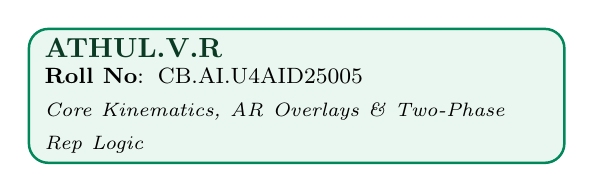
\begin{tikzpicture}
  \node[draw=BorderGreen, line width=0.9pt, fill=LightMint, rounded corners=7pt, 
        minimum width=68mm, minimum height=14mm, text width=64mm, align=left] {
    \textbf{\textcolor{DarkForest}{ATHUL.V.R}}\\
    \footnotesize \textbf{Roll No}: CB.AI.U4AID25005\\
    \scriptsize \textit{Core Kinematics, AR Overlays \& Two-Phase Rep Logic}
  };
\end{tikzpicture}

\vspace{3mm}

\begin{tikzpicture}
  \node[draw=BorderGreen, line width=0.9pt, fill=LightMint, rounded corners=7pt, 
        minimum width=68mm, minimum height=14mm, text width=64mm, align=left] {
    \textbf{\textcolor{DarkForest}{TVSS PHANINDRA GUPTA}}\\
    \footnotesize \textbf{Roll No}: CB.AI.U4AID25055\\
    \scriptsize \textit{Anti-Cheat Posture Lockout \& ADL Motor Task Engine}
  };
\end{tikzpicture}

\column{0.48\textwidth}

\begin{tikzpicture}
  \node[draw=BorderGreen, line width=0.9pt, fill=LightMint, rounded corners=7pt, 
        minimum width=68mm, minimum height=14mm, text width=64mm, align=left] {
    \textbf{\textcolor{DarkForest}{M VITTAL}}\\
    \footnotesize \textbf{Roll No}: CB.AI.U4AID25033\\
    \scriptsize \textit{Arcade Neuro-Games Arena \& Air-Canvas Drawing}
  };
\end{tikzpicture}

\vspace{3mm}

\begin{tikzpicture}
  \node[draw=BorderGreen, line width=0.9pt, fill=LightMint, rounded corners=7pt, 
        minimum width=68mm, minimum height=14mm, text width=64mm, align=left] {
    \textbf{\textcolor{DarkForest}{K NANDA KISHORE}}\\
    \footnotesize \textbf{Roll No}: CB.AI.U4AID25027\\
    \scriptsize \textit{Clinical Telemetry Reports, Backend API \& Testing}
  };
\end{tikzpicture}
\end{columns}
\end{frame}

% ==================== SLIDE 3 ====================
\begin{frame}{Table of Contents}
\vspace{-2mm}
\begin{columns}[T]
\column{0.48\textwidth}
\begin{block}{Phase I: Foundation \& Core Math}
\footnotesize
\renewcommand{\arraystretch}{1.12}
\begin{tabular}{clc}
\textbf{Sec} & \textbf{Topic} & \textbf{Page} \\
\midrule
\textbf{01} & Clinical Motivation \& Overview & 4 \\
\textbf{02} & System Architecture (4 Sessions) & 5 \\
\textbf{03} & Literature Review (4 Works) & 6 \\
\textbf{04} & Research Gaps \& Solution & 7 \\
\textbf{05} & Project Objectives & 8 \\
\textbf{06} & Methodology \& Modular Pipeline & 9 \\
\textbf{07} & Motion-Math: Real-Time (I) & 10 \\
\end{tabular}
\end{block}

\column{0.48\textwidth}
\begin{block}{Phase II: Protocols \& Validation}
\footnotesize
\renewcommand{\arraystretch}{1.12}
\begin{tabular}{clc}
\textbf{Sec} & \textbf{Topic} & \textbf{Page} \\
\midrule
\textbf{08} & Motion-Math: Real-Time (II) & 11 \\
\textbf{09} & Motion-Math: Anti-Cheat Gating & 12 \\
\textbf{10} & Motion-Math: Smoothness \& Audio & 13 \\
\textbf{11} & 9 Clinical Stroke Protocols & 14 \\
\textbf{12} & 7 Functional ADL Simulations & 15 \\
\textbf{13} & Experimental Validation (49 Tests) & 16 \\
\textbf{14} & Conclusion \& Live Demonstration & 17 \\
\end{tabular}
\end{block}
\end{columns}
\end{frame}

% ==================== SLIDE 4 ====================
\begin{frame}{01 · Project Idea — Introduction \& Overview}
\vspace{-1mm}
\begin{itemize}
    \setlength{\itemsep}{2.5pt}
    \item \textbf{Clinical Problem}: Stroke survivors experience severe loss of upper-limb, wrist, and fine-motor finger control.
    \item \textbf{Medical Principle}: Motor recovery relies on \textbf{neuroplasticity} via repetitive, biomechanically correct practice.
    \item \textbf{Current Limitations}: Manual goniometry is subjective, sensor suits are cost-prohibitive ($>\$1000$), and vision tools ignore fingers.
\end{itemize}

\vspace{1.5mm}
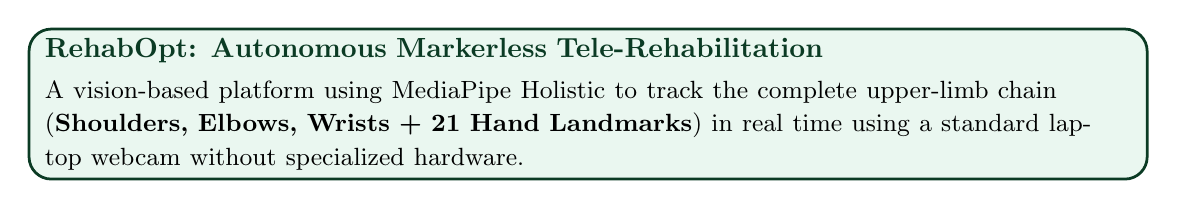
\begin{tikzpicture}
  \node[draw=DarkForest, line width=1pt, fill=LightMint, rounded corners=8pt, 
        minimum width=142mm, minimum height=16mm, text width=138mm, align=left] {
    \textbf{\textcolor{DarkForest}{RehabOpt: Autonomous Markerless Tele-Rehabilitation}}\\[1mm]
    \small A vision-based platform using MediaPipe Holistic to track the complete upper-limb chain (\textbf{Shoulders, Elbows, Wrists + 21 Hand Landmarks}) in real time using a standard laptop webcam without specialized hardware.
  };
\end{tikzpicture}

\vspace{1.5mm}
\begin{itemize}
    \item \textbf{Explainable Motion-Math Core}: 100\% deterministic mathematical goniometry and convex optimization without black-box ML biases.
\end{itemize}
\end{frame}

% ==================== SLIDE 5 ====================
\begin{frame}{02 · System Architecture \& 4 Unified Sessions}
\begin{columns}[T]
\column{0.48\textwidth}
\begin{block}{Session 1: Patient ID \& Security}
\begin{itemize}
    \setlength{\itemsep}{1pt}
    \item Auto-generated Patient IDs (\texttt{SP-00000000X}).
    \item SQLite database with password hashing \& streaks.
\end{itemize}
\end{block}

\vspace{2mm}
\begin{block}{Session 2: Clinical Dashboard}
\begin{itemize}
    \setlength{\itemsep}{1pt}
    \item One-click therapy launch for prescribed routines.
    \item Multimodal medical document parsing assistant.
\end{itemize}
\end{block}

\column{0.48\textwidth}
\begin{block}{Session 3: Interactive Therapy Arena}
\begin{itemize}
    \setlength{\itemsep}{1pt}
    \item \textbf{9 Clinical Exercises} with two-phase rep counting.
    \item \textbf{7 ADL Daily Tasks} \& \textbf{4 Arcade Games}.
    \item 3D neon air-canvas finger drawing therapy.
\end{itemize}
\end{block}

\vspace{2mm}
\begin{block}{Session 4: Telemetry \& Clinical Reports}
\begin{itemize}
    \setlength{\itemsep}{1pt}
    \item Real-time ROM goniometry \& 0--100 smoothness index.
    \item FFT tremor spectrum (4--12 Hz) \& exportable PDF.
\end{itemize}
\end{block}
\end{columns}
\end{frame}

% ==================== SLIDE 6 ====================
\begin{frame}{03 · Literature Review (4 Benchmark Works)}
\vspace{-2mm}
\centering
\setlength{\tabcolsep}{3pt}
\fontsize{7.5pt}{9.2pt}\selectfont
\renewcommand{\arraystretch}{1.08}
\begin{tabular}{p{2.3cm}p{1.9cm}p{3.2cm}p{3.1cm}p{2.5cm}}
\toprule
\textbf{Paper \& Author} & \textbf{Topic} & \textbf{Methodology} & \textbf{Reported Outcomes} & \textbf{Limitations} \\
\midrule
\textbf{UI-PRMD Dataset}\newline Vakanski et al. (2018)\newline \textit{IEEE Access} & 
Upper-body rehab exercise & 
10 healthy + 10 stroke subjects, Kinect v2, DTW \& LCS classification & 
100\% classification accuracy across 10 upper-body exercises & 
Needs Kinect sensor; body-only (no fingers); no live quality scoring. \\
\midrule
\textbf{KIMORE Dataset}\newline Capecci et al. (2019)\newline \textit{IEEE TNSRE} & 
Kinematic features for remote rehab & 
5 exercises across 77 subjects using Kinect v2; extracted angles \& ROM & 
Strong correlation between kinematic features and clinical scales & 
Dependent on Kinect; offline analysis only; no live patient biofeedback. \\
\midrule
\textbf{MediaPipe}\newline Lugaresi et al. (2019)\newline \textit{arXiv:1906.08172} & 
On-device perception framework & 
Graph-based pipeline for synchronized pose, hand, and face tracking & 
Real-time landmark inference on commodity hardware & 
General perception framework; lacks clinical logic and rep state machines. \\
\midrule
\textbf{Organizing Principle}\newline Hogan, N. (1984)\newline \textit{J. Neuroscience} & 
Mathematical model of smooth movement & 
Derived minimum-jerk trajectory by minimizing time-integral of squared jerk & 
Established minimum-jerk as standard model for voluntary reaching & 
Theoretical planar model; lacks vision integration and convex joint constraints. \\
\bottomrule
\end{tabular}
\end{frame}

% ==================== SLIDE 7 ====================
\begin{frame}{04 · Research Gap \& How We Fill It}
\begin{columns}[T]
\column{0.48\textwidth}
\begin{block}{Identified Gaps in Literature}
\begin{itemize}
    \setlength{\itemsep}{1.5pt}
    \item \textbf{Hardware Barrier}: Expensive sensors ($>\$1000$) prevent home deployment.
    \item \textbf{Torso-Only Tracking}: Existing tools ignore fine-motor wrist and fingers.
    \item \textbf{Lack of Form Guidance}: Patients exercise without ideal visual motion paths.
    \item \textbf{Subjective Progress}: Absence of numerical ROM and tremor isolation.
    \item \textbf{Therapy Fatigue}: Monotonous drills cause high dropout ($<30\%$).
\end{itemize}
\end{block}

\column{0.48\textwidth}
\begin{block}{How RehabOpt Fills the Gap}
\begin{itemize}
    \setlength{\itemsep}{1.5pt}
    \item \textbf{Zero Hardware Barrier}: Operates completely on standard laptop webcams.
    \item \textbf{Full Kinematic Chain}: Tracks shoulders, elbows, wrists, and 21 hand joints.
    \item \textbf{Real-Time Biofeedback}: Live skeleton pose guides and minimum-jerk curves.
    \item \textbf{Quantitative Telemetry}: Real-time 3D angles, 0--100 smoothness, and FFT spectra.
    \item \textbf{Gamified Dual Retraining}: 9 clinical drills + 7 ADL tasks + 4 reflex games.
\end{itemize}
\end{block}
\end{columns}
\end{frame}

% ==================== SLIDE 8 ====================
\begin{frame}{05 · Project Objectives}
\begin{columns}[T]
\column{0.48\textwidth}
\begin{block}{Core Perception \& Kinematics}
\begin{itemize}
    \setlength{\itemsep}{2pt}
    \item \textbf{Real-Time Edge Vision}: 60 FPS upper-body and 21 hand mesh tracking in-browser.
    \item \textbf{9 Clinical Stroke Protocols}: Shoulder, elbow, wrist, and fine-motor pincer drills.
    \item \textbf{Anti-Cheat Posture Lock}: Slope filter freezing exercises when trunk tilts $>25^\circ$.
    \item \textbf{Two-Phase State Machine}: 0.5 half-rep on hold + 1.0 full-rep on return.
\end{itemize}
\end{block}

\column{0.48\textwidth}
\begin{block}{Analytics \& Clinical Interface}
\begin{itemize}
    \setlength{\itemsep}{2pt}
    \item \textbf{Explainable Motion-Math}: 10 deterministic mathematical formulas.
    \item \textbf{Functional ADL Retraining}: 7 simulated daily living motor independence tasks.
    \item \textbf{Closed-Loop Biofeedback}: Auditory pitch-tone sonification (220--880 Hz).
    \item \textbf{Automated Telemetry}: Session analytics exported to clinical PDF report cards.
\end{itemize}
\end{block}
\end{columns}
\end{frame}

% ==================== SLIDE 9 ====================
\begin{frame}{06 · Methodology \& Modular Pipeline}
\begin{columns}[T]
\column{0.48\textwidth}
\begin{block}{1. Video Ingestion \& Tracking}
\begin{itemize}
    \setlength{\itemsep}{1pt}
    \item 30/60 FPS webcam frame capture.
    \item MediaPipe Holistic extracts 33 Pose + 21 Hand mesh landmarks in local WebAssembly worker.
\end{itemize}
\end{block}

\vspace{2mm}
\begin{block}{2. Motion-Math Kinematic Core}
\begin{itemize}
    \setlength{\itemsep}{1pt}
    \item Vector dot products calculate joint angles ($\theta$).
    \item Anti-cheat slope filter validates trunk posture.
\end{itemize}
\end{block}

\column{0.48\textwidth}
\begin{block}{3. Two-Phase Repetition Engine}
\begin{itemize}
    \setlength{\itemsep}{1pt}
    \item \textbf{Phase 1}: Target reach + isometric hold $\rightarrow$ \textbf{Half Rep (0.5)}.
    \item \textbf{Phase 2}: Controlled return to baseline $\rightarrow$ \textbf{Full Rep (1.0)}.
    \item 300ms hold grace window absorbs dropped frames.
\end{itemize}
\end{block}

\vspace{2mm}
\begin{block}{4. Feedback \& Clinical Reporting}
\begin{itemize}
    \setlength{\itemsep}{1pt}
    \item Web Audio API continuous ROM pitch sonification.
    \item Session telemetry compiled into exportable PDF report.
\end{itemize}
\end{block}
\end{columns}
\end{frame}

% ==================== SLIDE 10 ====================
\begin{frame}{07 · Mathematical Foundation — Real-Time Layer (Part 1)}
\begin{columns}[T]
\column{0.48\textwidth}
\begin{block}{C1 · Vector Geometry (Joint Angles)}
$$\theta = \arccos\left(\frac{\vec{a} \cdot \vec{b}}{\|\vec{a}\| \|\vec{b}\|}\right) \times \frac{180^\circ}{\pi}$$
\begin{itemize}
    \setlength{\itemsep}{2pt}
    \item \textbf{3D Joint Vectors}: $\vec{a} = \vec{P}_{\text{sh}} - \vec{P}_{\text{el}}$, $\vec{b} = \vec{P}_{\text{wr}} - \vec{P}_{\text{el}}$.
    \item \textbf{Application}: Calculates live elbow, wrist, and shoulder angles displayed on skeletal overlay.
    \item \textbf{Exercise Gating}: Extension $\ge 140^\circ \rightarrow$ Flexion return $< 125^\circ$.
\end{itemize}
\end{block}

\column{0.48\textwidth}
\begin{block}{C2 · Target Reaching ($L_2$ Distance)}
$$d = \sqrt{(\Delta x)^2 + (\Delta y)^2} \le r_{\text{target}}$$
\begin{itemize}
    \setlength{\itemsep}{2pt}
    \item \textbf{Reach Condition}: Target reached when $d \le r_{\text{target}}$, triggering visual state change and progress arc.
    \item \textbf{Application}: Measures fingertip/wrist distance to targets across all 9 exercises and 4 arcade games.
\end{itemize}
\end{block}
\end{columns}
\end{frame}

% ==================== SLIDE 11 ====================
\begin{frame}{08 · Mathematical Foundation — Real-Time Layer (Part 2)}
\begin{columns}[T]
\column{0.48\textwidth}
\begin{block}{C3 · Scale-Invariant Palm Dispersion}
$$\text{Spread Ratio} = \frac{\frac{1}{5}\sum_{i \in \{4,8,12,16,20\}} \|\vec{P}_i - \vec{P}_{\text{palm}}\|}{\|\vec{P}_9 - \vec{P}_0\|}$$
\begin{itemize}
    \setlength{\itemsep}{2pt}
    \item \textbf{Hand Shape Topology}: Normalized against palm scale $\|\vec{P}_9 - \vec{P}_0\|$ for child and adult size invariance.
    \item \textbf{Deterministic Gating}: Ratio $\le 0.95 \implies$ Closed Fist; Ratio $\ge 1.05 \implies$ Open Palm.
\end{itemize}
\end{block}

\column{0.48\textwidth}
\begin{block}{C4 · Tremor Isolation (Discrete FFT)}
$$X[k] = \sum_{n=0}^{N-1} x[n] \cdot e^{-j \frac{2\pi kn}{N}}$$
\begin{itemize}
    \setlength{\itemsep}{2pt}
    \item \textbf{Frequency Domain}: Converts wrist position buffer time-series into frequency spectra.
    \item \textbf{Pathological Isolation}: Detects power spikes in the clinical 4--12 Hz band for resting/action tremor analysis.
\end{itemize}
\end{block}
\end{columns}
\end{frame}

% ==================== SLIDE 12 ====================
\begin{frame}{09 · Mathematical Foundation — Anti-Cheat \& Motor Gating}
\begin{columns}[T]
\column{0.48\textwidth}
\begin{alertblock}{E1 · Anti-Cheat Trunk Lateral Tilt Angle}
$$\text{Tilt} = \left|\arctan2(\Delta y_{\text{sh}}, \Delta x_{\text{sh}})\right| \times \frac{180^\circ}{\pi}$$
\begin{itemize}
    \setlength{\itemsep}{2pt}
    \item \textbf{Trunk Posture Lock}: Evaluates inter-shoulder line slope in real time.
    \item \textbf{Lockout Freeze}: If $\text{Tilt} > 25^\circ$, session freezes: \textit{"Keep shoulders level"}. Exempted for shrugs.
\end{itemize}
\end{alertblock}

\column{0.48\textwidth}
\begin{block}{E2 · Scale-Invariant Pincer Grasp Ratio}
$$\text{Pinch Ratio} = \frac{\|\vec{P}_4 - \vec{P}_8\|}{\|\vec{P}_9 - \vec{P}_0\|}$$
\begin{itemize}
    \setlength{\itemsep}{2pt}
    \item \textbf{Fine-Motor Coordination}: Gap between thumb tip (4) and index tip (8).
    \item \textbf{Two-Phase Gating}: Ratio $\le 0.32$ (Pinch locked) $\rightarrow$ Ratio $\ge 0.40$ (Release wide). Size invariant.
\end{itemize}
\end{block}
\end{columns}
\end{frame}

% ==================== SLIDE 13 ====================
\begin{frame}{10 · Mathematical Foundation — Analytical \& Biofeedback}
\begin{columns}[T]
\column{0.48\textwidth}
\begin{block}{S1 \& E3 · Smoothness \& Wrist Pitch}
$$\text{Score} = 100 - \min\left(100, 20\log_{10}\left(\frac{\frac{1}{2}\int \text{Jerk}^2 dt \cdot T^5}{D^2}\right)\right)$$
\begin{itemize}
    \setlength{\itemsep}{1pt}
    \item Jerk computed via discrete finite differences $\frac{d^3x}{dt^3}$.
    \item \textbf{E3 Wrist Pitch}: $\text{Pitch} = \arctan2(\Delta y_{\text{h}}, \Delta x_{\text{h}}) \times \frac{180^\circ}{\pi}$. Upward $\ge 14^\circ \rightarrow$ level return $\le 10^\circ$.
\end{itemize}
\end{block}

\column{0.48\textwidth}
\begin{block}{B1 \& P1 · Audio Pitch \& Pursuit}
$$f(\theta) = f_{\min} + \left(\frac{\theta - \theta_{\min}}{\theta_{\max} - \theta_{\min}}\right)(f_{\max} - f_{\min})$$
\begin{itemize}
    \setlength{\itemsep}{1pt}
    \item Live ROM mapped continuously to 220--880 Hz tones.
    \item \textbf{P1 Harmonic Pursuit}: $X(t) = 0.50 + 0.28\sin(0.65t)$, $Y(t) = 0.48 + 0.08\sin(1.30t)$ with 10s countdown.
\end{itemize}
\end{block}
\end{columns}
\end{frame}

% ==================== SLIDE 14 ====================
\begin{frame}{11 · Final Implementation: 9 Clinical Exercises Protocol}
\vspace{-2mm}
\centering
\setlength{\tabcolsep}{3pt}
\fontsize{7.5pt}{9.2pt}\selectfont
\renewcommand{\arraystretch}{1.06}
\begin{tabular}{cp{3.4cm}p{2.6cm}p{4.2cm}c}
\toprule
\textbf{\textcolor{DarkForest}{\#}} & 
\textbf{\textcolor{DarkForest}{Clinical Exercise}} & 
\textbf{\textcolor{DarkForest}{Target Joints}} & 
\textbf{\textcolor{DarkForest}{Validation Threshold \& State Transition}} & 
\textbf{\textcolor{DarkForest}{Hold}} \\
\midrule
\textbf{1} & Elbow Extension \& Flexion & Shoulder, Elbow, Wrist & Angle $\ge 140^\circ$ (Half Rep 0.5) $\rightarrow$ Flex $< 125^\circ$ (Full 1.0) & 0.6s \\
\textbf{2} & Shoulder Elevation (Shrug) & Left / Right Shoulders & Shrug lift $\ge 3.5\%$ screen $\rightarrow$ Return to resting baseline & 1.2s \\
\textbf{3} & Hand Open \& Close & 21 Finger Landmarks & Tight fist $\le 0.95$ $\rightarrow$ Open palm dispersion $\ge 1.05$ & 0.4s / 0.5s \\
\textbf{4} & Horizontal Wrist Up/Down & Wrist, Index Knuckle & Cock wrist UP $\ge 14^\circ \rightarrow$ Return level $\le 10^\circ$ & 0.5s \\
\textbf{5} & Diagonal Reach \& Hold & Shoulder, Elbow, Wrist & Intercept diagonal AR waypoint + maintain steady hold & 2.0s \\
\textbf{6} & Two-Target Horizontal Glide & Shoulder, Elbow, Wrist & Glide to Station 2 $\rightarrow$ Glide return to Station 1 & 0.6s / 0.6s \\
\textbf{7} & Open Palm L/R Rotation & Wrist, Palm Center & Knuckle lateral shift $<-0.035 \rightarrow >0.035$ & 0.4s / 0.4s \\
\textbf{8} & Dynamic Moving Pursuit & Upper Limb Chain & Continuous harmonic sinusoidal pursuit with 10s countdown & 10.0s \\
\textbf{9} & Virtual Pincer Grasp & Thumb (4), Index (8) & Pincer pinch $\le 0.32$ (Pinch locked) $\rightarrow$ Release wide $\ge 0.40$ & 0.5s \\
\bottomrule
\end{tabular}
\end{frame}

% ==================== SLIDE 15 ====================
\begin{frame}{12 · ADL Lab: 7 Functional Daily Living Simulations}
\begin{columns}[T]
\column{0.48\textwidth}
\begin{block}{Functional Daily Living Tasks (1--4)}
\begin{enumerate}
    \setlength{\itemsep}{2pt}
    \item \textbf{Balloon Pump}: Open grasp + closed fist pumping.
    \item \textbf{Water Reservoir}: Cupped palm water transfer.
    \item \textbf{Light Switch}: Ballistic upward wrist flick.
    \item \textbf{ATM PIN Pad}: Index fingertip 90px hit-boxes.
\end{enumerate}
\end{block}

\column{0.48\textwidth}
\begin{block}{Fine-Motor \& Elevation Tasks (5--7)}
\begin{enumerate}
    \setcounter{enumi}{4}
    \setlength{\itemsep}{2pt}
    \item \textbf{Pour the Water}: Forearm pronation tilt tracking.
    \item \textbf{Cup Shelf Lift}: Grasp cup, vertical elevation, shelf.
    \item \textbf{Clean Window Dust}: Index scrubbing coverage $\ge 90\%$.
\end{enumerate}
\vspace{1mm}
\textit{+ 4 Neuro-Arcade Games \& 3D Neon Air-Canvas.}
\end{block}
\end{columns}
\end{frame}

% ==================== SLIDE 16 ====================
\begin{frame}{13 · Experimental Validation \& Test Results}
\vspace{-2mm}
\centering
\setlength{\tabcolsep}{6pt}
\small
\renewcommand{\arraystretch}{1.10}
\begin{tabular}{lccc}
\toprule
\textbf{\textcolor{DarkForest}{Verification Suite}} & 
\textbf{\textcolor{DarkForest}{Tests Executed}} & 
\textbf{\textcolor{DarkForest}{Pass Rate}} & 
\textbf{\textcolor{DarkForest}{Status}} \\
\midrule
\textbf{Clinical Exercises (Phase 1/2 Reps)} & 13 & 100\% (13 / 13) & \textbf{PASSED} \\
\textbf{ADL Kinematic Motor Engine} & 12 & 100\% (12 / 12) & \textbf{PASSED} \\
\textbf{Backend Security \& Telemetry API} & 24 & 100\% (24 / 24) & \textbf{PASSED} \\
\midrule
\textbf{Total Automated System Validations} & \textbf{49} & \textbf{100\% (49 / 49)} & \textbf{ALL PASSED} \\
\bottomrule
\end{tabular}

\vspace{2mm}
\begin{columns}[T]
\column{0.48\textwidth}
\begin{block}{System Performance Telemetry}
\begin{itemize}
    \item \textbf{AR Render Rate}: Sustained 60 FPS in browser.
    \item \textbf{CV Latency}: 0 ms network lag (WebAssembly).
    \item \textbf{Anti-Cheat Gating}: 0\% unpenalized lean cheats.
\end{itemize}
\end{block}

\column{0.48\textwidth}
\begin{block}{Platform Reliability Verified}
\begin{itemize}
    \item All 7 core web routes return HTTP 200 OK.
    \item Zero NaN coordinates or math overflow errors.
    \item Automated session export to clinical PDF report.
\end{itemize}
\end{block}
\end{columns}
\end{frame}

% ==================== SLIDE 17 ====================
\begin{frame}{14 · Conclusion \& Key Clinical Impact}
\begin{block}{Key Contributions \& Takeaways}
\begin{itemize}
    \setlength{\itemsep}{3.5pt}
    \item \textbf{▶ Hardware Democratization}: Eliminates expensive $\$1000+$ sensor suits; full upper-limb tele-rehabilitation runs on standard laptop webcams.
    \item \textbf{▶ Complete Kinematic Chain}: Synchronous tracking of shoulders, elbows, wrists, and all 21 hand landmarks.
    \item \textbf{▶ 100\% Explainable Math Core}: Replaces opaque black-box deep learning with verifiable vector geometry, convex formulations, and 10 core formulas.
    \item \textbf{▶ Repetition Integrity}: Milestone-locked half-reps (0.5) and full-reps (1.0) with anti-cheat trunk tilt prevention guarantee genuine therapeutic progress.
    \item \textbf{▶ Maximized Engagement}: Combines 9 clinical exercises, 7 functional ADL tasks, 4 arcade games, 3D air-canvas, and real-time audio biofeedback.
\end{itemize}
\end{block}
\end{frame}

% ==================== SLIDE 18 ====================
\begin{frame}[plain]
\begin{tikzpicture}[remember picture, overlay]
  % Top green rule
  \fill[TopGreen] (current page.north west) rectangle ([yshift=-1.4mm]current page.north east);
  % Central mint card
  \node[draw=DarkForest, line width=1.2pt, fill=LightMint, rounded corners=12pt, 
        minimum width=132mm, minimum height=60mm, text width=124mm, align=center] 
        at (current page.center) {
    {\Large \textbf{\textcolor{DarkForest}{RehabOpt-AR}}}\\[1.5mm]
    {\large \textbf{\textcolor{DarkForest}{Interactive Vision-Based AR Suite for Stroke Recovery}}}\\[3mm]
    \textcolor{TopGreen}{\rule{90mm}{1pt}}\\[3mm]
    {\normalsize \textbf{\textcolor{DarkForest}{Department of Artificial Intelligence}}}\\[3mm]
    {\Huge \textbf{\textcolor{DarkForest}{Thank You!}}}\\[3mm]
    {\normalsize \textbf{\textcolor{DarkForest}{Questions \& Live Demonstration}}}
  };
\end{tikzpicture}
\end{frame}

\end{document}
